\documentclass[tikz,border=10pt]{standalone}
\usetikzlibrary{calc}
\begin{document}
% Scale s = 0.010855 cm per px; origin at O (424.6,686.1 px); y flipped.
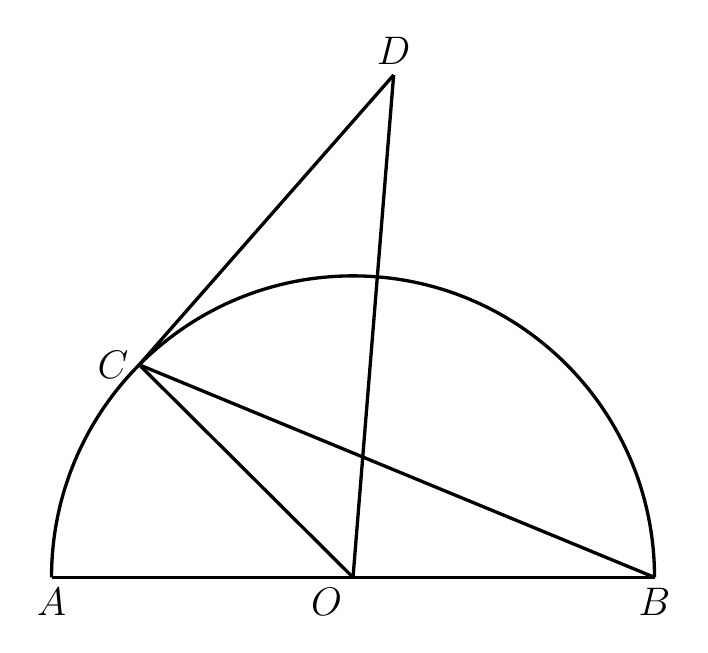
\begin{tikzpicture}[line width=1.2pt, line join=round]
  % Named coordinates (cm)
  \coordinate (O) at (0,0);
  \coordinate (A) at (-3.829,0);
  \coordinate (B) at (3.829,0);
  \coordinate (C) at (-2.715,2.700);
  \coordinate (D) at (0.516,6.380);

  % Upper semicircle from A through the top to B (radius 3.829 cm)
  \draw (A) arc[start angle=180, delta angle=-180, radius=3.829];

  % Segments
  \draw (A) -- (B);
  \draw (O) -- (D);
  \draw (D) -- (C);
  \draw (C) -- (B);
  \draw (O) -- (C);

  % Labels
  \node[below] at (A) {\fontsize{13.5}{16.2}\selectfont $A$};
  \node[below] at (B) {\fontsize{13.5}{16.2}\selectfont $B$};
  \node[below left] at (O) {\fontsize{13.5}{16.2}\selectfont $O$};
  \node[left] at (C) {\fontsize{13.5}{16.2}\selectfont $C$};
  \node[above] at (D) {\fontsize{13.5}{16.2}\selectfont $D$};
\end{tikzpicture}
\end{document}